\documentclass[tikz,border=3.14mm]{standalone}
\begin{document}
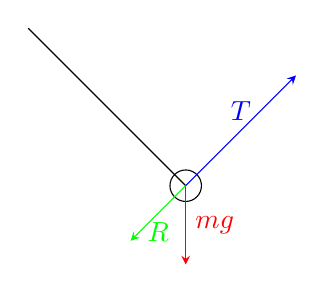
\begin{tikzpicture}

% Draw the pendulum string
\draw (0,0) -- (2,-2);
% Draw the pendulum bob
\draw (2,-2) circle (0.2cm);

% Draw and label the gravitational force
\draw[red,-stealth] (2,-2) -- ++(0,-1) node[midway,right] {$mg$};

% Draw and label the tension
\draw[blue,-stealth] (2,-2) -- ++(1.4,1.4) node[midway,above] {$T$};

% Draw and label the air resistance
\draw[green,-stealth] (2,-2) -- ++(-0.7,-0.7) node[midway,below] {$R$};

\end{tikzpicture}
\end{document}